\documentclass[12pt]{article}
\usepackage[utf8]{inputenc}

\usepackage[margin = 0.7in]{geometry}
\usepackage{amsmath}
\usepackage{amsfonts}
\usepackage{amssymb}
\usepackage{amsthm}
\usepackage{graphicx}
\usepackage{placeins}
\usepackage{enumitem}
\usepackage{dsfont}
\usepackage{booktabs}

\newcommand{\N}{\mathbb{N}}
\newcommand{\Z}{\mathbb{Z}}
\newcommand{\R}{\mathbb{R}}
\newcommand{\E}{\mathbb{E}}
\newcommand{\Q}{\mathbb{Q}}
\newcommand{\de}{\mathrm{d}}
\newcommand{\one}{\mathds{1}}

\title{ECON 899: Problem Set 3}
\author{Katherine Kwok\footnote{I collaborated with Anya Tarascina and Claire Kim on this assignment.}}
\date{October 2021}

\begin{document}

\maketitle
\noindent \textbf{Overview: } For this assignment, the goal is to replicate a simple version of the Conesa and Krueger (1999) model. Using this model, we then evaluate the impacts of eliminating Social Security in the U.S. \\\\
% Part 1
\noindent \textbf{Exercise 1: Dynamic Programming Problem} \\\\
First, we set up and solve the dynamic programming problem for retirees and workers. Since we have a finite time horizon, we can iterate from the final period of life backwards to the first period. For the first two exercises, we are given wage, interest rate, and social security benefit ($w = 1.05, r = 0.05, b = 0.2$), in addition to other parameter values. \\\\
The plot below displays the value function for an agent at model-age 50. We can observe that the value function is increasing and concave over the current asset level. 

\begin{figure}[!htbp]
    \centering
    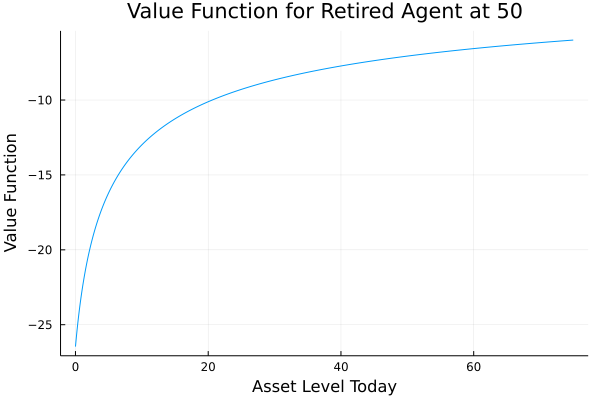
\includegraphics[width = 0.8\textwidth]{age_50_value_func.png}
    \caption{Value Function for Model-Age 50}
    \label{fig:val_func_50}
\end{figure}

\begin{figure}[!htbp]
    \centering
    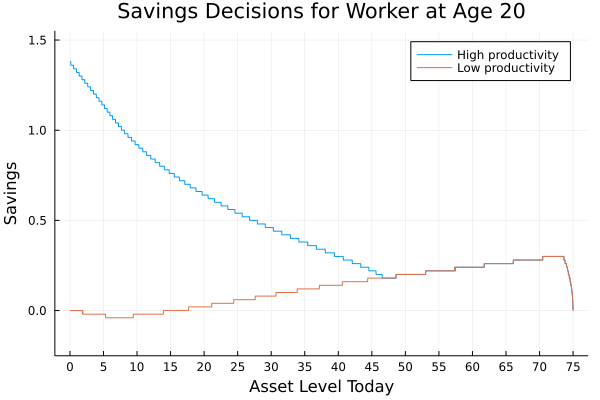
\includegraphics[width = 0.8\textwidth]{age_20_savings.png}
    \caption{Savings Decisions for Model-Age 20}
    \label{fig:savings_20}
\end{figure}

\noindent Next, we plot the savings decisions for workers, separating out high productivity from low productivity states. As shown in the plot above, the savings amount depends on both $z$ (productivity) and $a$ (current asset level). For high productivity individuals, savings is decreasing in current asset level until around asset level 45, then the line slopes upward. For low productivity individuals, savings is generally increasing in current asset level, except between asset levels 0 - 10. For both workers, savings drops quickly between asset levels 70 - 75. \\\\
The relevant code for this exercise is in the ``main\_program.jl" file (lines 26 - 30) and the ``models\_and\_functions.jl" file (lines 168 - 332).\\\\


% Part 2
\noindent \textbf{Exercise 2: Steady-State Distributions} \\\\ Once we are able to solve the individual dynamic programming problem, we have the price-specific value function, policy function (in terms of asset), and labor supply function. Then, we can compute the stationary distribution of agents across ages, productivity states, and asset holdings. Basically, these distributions allow us to map an individual from this period to the next period, given the state in this period. We can iterate forward to solve for the stationary distribution, starting with the ergodic distribution of high and low productivities $(0.2037, 0.7963)$. We assume as model-age 1 agents start with zero assets. \\\\
The relevant code for this exercise is in the ``main\_program.jl" file (lines 32 - 36) and the ``models\_and\_functions.jl" file (lines 333 - 398). We call this steady-state distribution $\psi$ in the code.\\\\

% Part 3
\noindent \textbf{Exercise 3: Benchmark Model and Experiments} \\\\
Using the algorithms we can built in exercises 1 and 2, we can then find equilibrium prices that solve the simplified version of the Conesa-Kruger model. While exercises 1 and 2 are based on given prices ($w$, $r$), we now solve for the equilibrium prices and associated aggregate capital and labor ($K, L$) using the ``guess and verify" method. \\\\
For a given $K_0 = K_{initial}, L_0 = L_{initial}$, we can find the prices and pension benefit levels:
\begin{align*}
    w_0 &= \frac{\partial}{\partial L} F(K, L) = \frac{\partial}{\partial L} K^{\alpha}L^{1-\alpha} = (1-\alpha) K^{\alpha} L^{-\alpha}
    \\
    r_0 &= \frac{\partial}{\partial K} F(K, L) - \delta = \frac{\partial}{\partial K} K^{\alpha}L^{1-\alpha} - \delta = \alpha K^{\alpha -1} L^{1-\alpha} - \delta\\
    b_0 &= \frac{\theta w_0 L_0}{\sum_{j = J^R}^N \mu_j}
\end{align*}
where $J^R$ is retirement age, $N$ is the total number of periods in life, and $\sum_{j = J^R}^N \mu_j$ is the share of retirees in the population. \\\\
Then, the prices are used to solve the individual dynamic programming problem and the steady-state distribution across ages, productivity states, and current asset levels. Using the resulting labor supply function $l_j(z, a)$ and stationary distribution $\psi_j(z, a)$, we can then calculate the new aggregate capital and labor $K_1, L_1$:
\begin{align*}
    K_1 &= \sum_{j=1}^N \sum_{a = a_1}^{a_{na}} \sum_{z \in \{z_l, z_h\}} \psi_j(z, a)a \\
    L_1 &= \sum_{j=1}^{J^R -1} \sum_{a = a_1}^{a_{na}} \sum_{z \in \{z_l, z_h\}} \psi_j(z, a) e(z, \eta_j) l_j(z, a)
\end{align*}
Finally, if the absolute differences between $K_0$ and $K_1$, and between $L_0$ and $L_1$ is within a tolerance value, we have converged. If not, we update $K_0 = \lambda K_1 + (1-\lambda)K_0$ and $L_0 = \lambda L_1 + (1-\lambda)L_0$. Then, we repeat the same process until convergence. \\\\
Using the algorithm above, we test six different scenarios for exercise 3 to evaluate the impact of the Social Security program on macroeconomic indicators: 
\begin{enumerate}
    \item Benchmark model with social security ($\theta = 0.11$)
    \item Benchmark model without social security ($\theta = 0$)
    \item Model with no idiosyncratic risks ($z_h = z_l = 0.5$) and social security ($\theta = 0.11$)
    \item Model with no idiosyncratic risks ($z_h = z_l = 0.5$) and no social security ($\theta = 0$)
    \item Model with exogenous labor supply ($\gamma = 1$) and social security ($\theta = 0.11$)
    \item Model with exogenous labor supply ($\gamma = 1$) and no social security ($\theta = 0$)
\end{enumerate}
\pagebreak
The results are summarized in the table below. 
\begin{center}
% Please add the following required packages to your document preamble:
% \usepackage{booktabs}
\begin{table}[!htbp]
\small
\begin{center}
\caption{Experiment Results} \medskip
\begin{tabular}{@{}lcccccc@{}}
\toprule
Scenario & BM         & BM + No SS & No risk    & No risk + No SS & Exog. LS   & Exog. LS + No SS \\ \midrule
$\theta$            & 0.11       & 0          & 0.11       & 0               & 0.11       & 0                \\
$z_h$             & 3          & 3          & 0.5        & 0.5             & 3          & 3                \\
$\gamma$            & 0.42       & 0.42       & 0.42       & 0.42            & 1          & 1                \\
\midrule
K                & 3.3589     & 4.6035     & 1.0453     & 1.2878          & 7.3598     & 10.4539          \\
L                & 0.3432     & 0.3652     & 0.16       & 0.1682          & 0.7543     & 0.7543           \\
w                & 1.4548     & 1.5936     & 1.2578     & 1.3317          & 1.4533     & 1.649            \\
r (\%)               & 2.36     & 1.11      & 4.83     & 3.79          & 2.38     & 0.69           \\
b                & 0.2251     & 0          & 0.0908     & 0               & 0.4942     & 0                \\
welfare          & -35.768    & -37.382    & -45.066    & -45.157         & -23.003    & -25.758          \\
cv(wealth)       & 1.5298     & 1.3983     & 0.6627     & 0.7603          & 1.5101     & 1.3243           \\
\midrule
iterations       & 11         & 6          & 11         & 12              & 9          & 3                \\
time             & 550 sec    & 307 sec    & 461 sec    & 526 sec         & 387 sec    & 127 sec          \\
$\lambda$           & 0.99       & 0.99       & 0.3        & 0.3             & 0.99       & 0.99             \\
tolerance        & 1.00e-03   & 1.00e-03   & 1.00e-02   & 1.00e-02        & 1.00e-03   & 1.00e-03         \\
initial K, L     & (3.3, 0.3) & (3.3, 0.3) & (1.0, 0.1) & (1.0,0.1)       & (3.0, 0.3) & (3.0, 0.3)       \\ \bottomrule
\end{tabular}
\end{center}
\label{tab} \par \medskip
{\footnotesize \textit{Notes: } The top section of the table summarizes input parameter values. The middle section summarizes the results for the particular scenario. The bottom section summarizes parameters and results related to run time and convergence speed. The $\lambda$ value, initial $K, L$, and tolerance control how quickly the program converges.}
\end{table}
\end{center}

%first exp
\noindent First, we solve the benchmark model without and without social security. This corresponds to the first two columns in the table above. The interest rate is 2.36\% in the benchmark model. The growth rate is around 1.1\%. Since the interest rate is greater than the growth rate, the economy is dynamically efficient according to the criterion developed by Abel, Mankiw, Summers and Zeckhauser (1989). \\\\
When social security is eliminated from the benchmark model, we see that aggregate capital and labor supply both increase. Aggregate capital goes from around 3.36 to 4.60, while aggregate labor supply goes from 0.343 to 0.365. This makes intuitive sense, since workers have to work more and save more, in order to have enough assets saved for consumption when they are retired. Without social security, aggregate welfare decreases from -35.77 to -37.28, so the population is worse off on average. However, not everyone is worse off when social security is eliminated. Younger workers are likely to be better off without social security, since they are not as concerned about working more and saving for retirement as older workers. Older workers are worse off for the aforementioned reason, and retirees are also worse off without the social security benefits. Also, cross sectional inequality decreases, as the coefficient of variation for wealth decreases from 1.53 to 1.40. \\\\
% second exp
The second set of experiments test the elimination of idiosyncratic productivity shocks with and without social security. To do so, we set the high productivity and low productivity to be the same (i.e. $z_h = z_l = 0.5$). This corresponds to the third and fourth column in the results table above. Looking at the scenario without idiosyncratic risk but with social security (column 3), aggregate capital is lower (1.05) compared to the benchmark (3.36). This indicates that agents use saving as an insurance against productivity shocks, in order to smooth their consumption. Thus, when there are no idiosyncratic shocks to productivity, savings decrease. \\\\
When social security is eliminated from the model without productivity shocks, we see that welfare decreases slightly from -45.07 to -45.16. This drop in welfare is smaller than the amount when social security is eliminated from the benchmark model. In the benchmark case, welfare drops from -35.77 to -37.38. This tells us that social security is a useful buffer against idiosyncratic shocks. These comparisons across steady state welfare levels are useful, but they do not give us the full picture of how welfare changes, as we don't know what welfare is along the transition path. \\\\
%third exp
In the third and final set of experiments, we make labor supply exogenous by setting $\gamma = 1$, and check the results with and without social security. When labor supply is exogenous, the aggregate labor supply remains the same (around -0.7543) with and without social security. This contrasts with the first set of experiments on the benchmark model, where aggregate labor supply increases from 0.343 to 0.365 when social security is eliminated. This suggests that social security has a distortionary effect on labor supply. Specifically, the tax on labor supply (levied to fund social security) decreases labor supply.





\end{document}

